\chapter{Architectural Views}

\section{Context View}

\subsection{Stakeholders' uses of this view}

\subsection{Context Diagram}

\begin{figure}[H]
    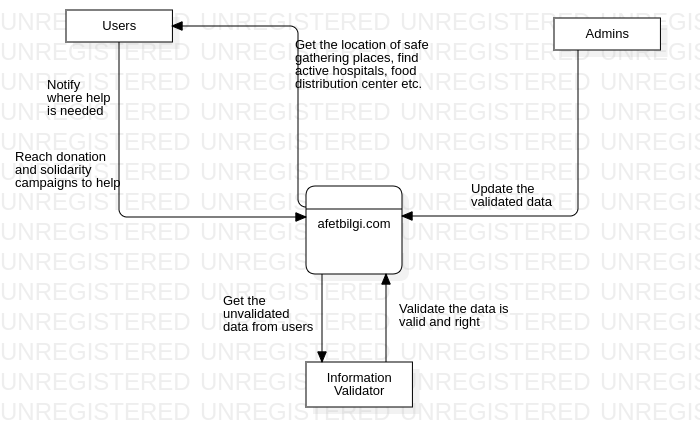
\includegraphics[scale = 0.6]{assets/Context Diagram.png}
    \caption[Context Diagram for afetbilgi.com]{Context Diagram for afetbilgi.com}
\end{figure}

As it can be observed from the context diagram, the system interacts with 3 external entities. These are users, admins and information validators. Afetbilgi.com users can use this website for 2 purpose. It can be used to deliver help or it can be used to get help who are affected by the disaster.
in addition to that, information validator gets the all information which delivered to them and by reaching the authorities validates the information. In meanwhile, admins update the database with these validated datas in the system. 

\subsection{External Interfaces}

\subsection{Interaction scenarios}

\section{Functional View}

\subsection{Stakeholders' use of this view}

\subsection{Component Diagram}

\subsection{Internal Interfaces}

\subsection{Interaction Patterns}

\section{Information View}

\subsection{Stakeholders' uses of this view}

\subsection{Database Class Diagram}

\subsection{Operations on Data}

\section{Deployment View}

\subsection{Stakeholders' uses of this view}

\subsection{Deployment Diagram}

\section{Design Rationale}